\documentclass[10pt,titlepage,letterpaper]{article}

\usepackage[utf8]{inputenc}
\usepackage{amsmath}
\usepackage{mathtools}
\usepackage{enumitem}
\usepackage{tikz}
\usepackage{graphicx}
\usepackage{subcaption}
\usepackage[nottoc]{tocbibind}
\usepackage{cite}

\begin{document}
	\setlength{\parskip}{1em}
	\title{An Approximate Solution to the Packing Problem With Respect to Knolling Applications}
	\author{Gerald Wu}
	\maketitle
	\pagenumbering{roman}
	\tableofcontents
	\newpage
	\pagenumbering{arabic}

	\section{Background}
	\subsection{Context}
	Knolling began in 1987, with a janitor of Frank Gehry's shop. Frank Gehry designed furniture for a company called Knoll. The janitor, named Andrew Kromelov, started arranging his tools at 90 degree angles and taking pictures of them because he found it aesthetically pleasing. As a tribute to the company he was working for, he named this process knolling\cite{knolling}.
	\subsection{Current Solutions}
	In my research, I found that there are currently no existing programs that automatically generate a knolling layout. There exist programs that pack rectangles in general as proof-of-concept approximate solutions to the packing problem\cite{tilings}. However, these do not exactly meet the criteria of a knolling program.
	\subsection{Problems with Current Solutions}
	No current solutions to this problem exist in the form that is easily usable by photography enthusiasts that wish to knoll. The few solutions that are semi-related require a non-trivial amount of programming and system administration skill in order to use. As this is meant for photographers, it is not appropriate to assume this level of computer knowledge from all members of the target audience.\par
	In addition, the traditional bin packing problem is an NP-hard problem. Since the knolling process sees very little benefit from exact solutions to the packing problem, it is extremely inefficient and computationally expensive to solve for an exact solution when an approximate solution is adequate.
	\subsection{Goals of Research}
	This project was performed in order to remedy the lack of knolling layout generators. Many advertisers use knolling to display products in an appealing way. Since the hardest part of knolling is coming up with an adequate layout, this program was created in order to simplify the process of knolling, for both casuals and professionals.

	\section{Methodology}
	\subsection{Approach}
	\subsubsection{Difference between traditional packing problem}
	I approached this problem with a traditional approximate packing problem solution. However, there is a fundamental difference between the traditional packing problem and the problem of knolling. Packing problems focus on packing a preset number of objects into a preset size bin. A crucial aspect of my problem is not a preset size, but a preset aspect ratio. Given a certain aspect ratio, the program must determine the smallest possible enclosing box that the objects can fit in.
	\subsubsection{Main program}
	The program first reads in a desired aspect ratio from the user. Using this aspect ratio, it determined the minimum possible guaranteed area to fit all the boxes. The minimum area was calculated by finding the perimeter of the trivial solution, and determining the dimensions of an enclosing rectangle using the same perimeter and the given aspect ratio.\par
	From here, the rectangles were packed using the sorted first-fit algorithm from left-to-right, top-to-bottom\cite{first-fit}. If the rectangles fit, then the length and width were decreased while preserving the aspect ratio and the rectangles were packed again. This process was repeated until the enclosing box was so small that the rectangles could not be packed. The last possible packing was the smallest possible packing determined by the program, and this configuration was written to an external file.\par
	After this is completed, the remaining whitespace on the sides is trimmed. This means that the final enclosing box is not truly the same aspect ratio as the one given, but it is instead a very close approximation. 
	\subsubsection{Helper program}
	A helper script written in bash was used to put finishing touches on the program. The bash script provided a simple user input to specify the number of rectangles wanted, as well as the desired aspect ratio. After passing these parameters to the main program, it reads the configuration file the main program generated. Using the ImageMagick program, it then creates a simple visual representation of the rectangle configuration.
	\subsection{Data Sets}
	To test data sets, I wrote a program to randomly generate rectangles and output them to a configuration file. Every time the main program runs, it reads this configuration file and attempts to pack them into the smallest possible enclosing rectangle. The set of rectangles can also be manually created to test specific configurations with known exact solutions.
	\subsection{Software}
	\begin{itemize}
		\item Main program: C++
		\item Helper programs
		\begin{itemize}
			\item Bash: Initialization program
			\item ImageMagick: Image manipulation program
			\item Feh: Standard image viewing program
		\end{itemize}
	\end{itemize}
	\subsection{Libraries}
	The only libraries used in this project were the standard C++ libraries: string and vector. The rectangle class was written by hand with no external libraries.
	\subsection{Hardware}
	No hardware outside of a computer was needed for this project --- it was entirely a software project.

	\section{Results}
	\subsection{What Happened}
	After many failed collision detections and far less than ideal algorithms, the project did eventually adequately tile the given rectangles into the smallest possible enclosing rectangle that matched the given aspect ratio. It is clearly not a perfect solution --- however, it did generate some close approximate solutions.
	\begin{figure}[ht]
		\centering
		\begin{subfigure}{0.40\textwidth}
			\centering
			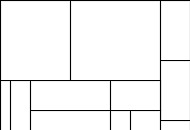
\includegraphics[height=3cm]{img/12.jpg}
			\caption{An example using 12 randomly generated rectangles.}
		\end{subfigure}
		\begin{subfigure}{0.40\textwidth}
			\centering
			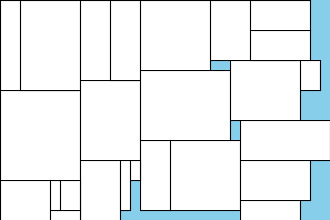
\includegraphics[height=3cm]{img/25.jpg}
			\caption{An example using 25 randomly generated rectangles.}
		\end{subfigure}
		\caption{Example outputs}
	\end{figure}
	\subsection{What Worked}
	The program can successfully read in rectangle configurations from files, and work with an arbitrary number of rectangles and aspect ratios. I've successfully tested up to 100 blocks, which is more than enough for the vast majority of practical applications of this program. I'm confident that this program will also work past 100 blocks given enough computation time.
	\subsection{What Didn't Work}
	The program does not have a function to read in user-specified images. This is not terribly difficult to implement, however, I ran out of time before I could implement it. It is also not fundamentally important to the core functionality of the program, so the program can still run and give significant results without this feature.\par
	Rotation was also not implemented in this program. While in some cases it would've saved a non-negligible amount of space, it would have been computationally expensive to implement.
	\subsection{Notable Observations}
	While running the program, I noticed that it ran much slower as the number of rectangles increased. I estimated the runtime to be around $\mathcal{O}(N^{10})$, so this would explain its rapid increase in time.\par
	In addition, the program appeared to produce less than ideal results towards the right of the generated image. While the left was almost an exact solution, the right would sometimes leave non-negligible gaps. This was probably due to a limitation of the sorted first-fit algorithm. Since I packed the rectangles from left-to-right, this caused the right side to sometimes become less than ideal.

	\section{Conclusion}
	\subsection{What Does It All Mean?}
	The packing problem has a fair amount of practical applications. Examples include CSS styling on websites and packing items for shipment. With enough effort, more optimal solutions can be found. Even though my program works and can provide approximate solutions to the application of knolling, a more optimized solution could be implemented with lesser hardware.
	\subsection{Status of the Problem}
	The goal of applying approximate packing problem solutions to the knolling problem was accomplished at a core level. The configuration generated, while not an exact solution, is adequate in most scenarios. It creates a visual representation of the solution.\par
	The ability to rotate each rectangle is missing. I decided to forgo this feature, as it would've added a significant amount of computation to an already computationally heavy program.
	\subsection{Unknowns}
	The ability of other algorithms is still unknown, as I was only able to implement one algorithm, the sorted first-fit algorithm. Other algorithms may have proven to be slightly more effective approximate solutions to the packing problem.
	\subsection{Improvements}
	Using the method of k-d trees to store the rectangles would've been significantly more efficient than creating a rudimentary rectangle data structure. The k-d trees approach to the rectangle data structure is more abstract and clever, and decreases what is currently an $\mathcal{O}(N^5)$ problem to $\mathcal{O}(NlogN)$. I attempted this approach for a few weeks, but couldn't get it to work. This is an excellent starting point to drastically reduce computation time for anyone looking to improve upon the program.\par
	In addition, the algorithm itself could be improved. In the paper \textit{A Thousand Ways to Pack the Bin --- A Practical Approach to Two-Dimensional Rectangle Bin Packing}\cite{thousand}, Jyl{\"a}nki extensively listed effective algorithms. Many of these could be applied to this program to achieve different results. In certain cases, they will produce better results than the sorted first-fit algorithm used in this project.

	\bibliographystyle{unsrt}
	\bibliography{references}

\end{document}
